\documentclass[12pt,a4paper]{article}
\usepackage[utf8]{inputenc}
\usepackage[russian]{babel}
\usepackage[OT1]{fontenc}
\usepackage{amsmath}
\usepackage{amsfonts}
\usepackage{amssymb}
\usepackage{graphicx}
\graphicspath{{Images/}}
\usepackage[left=2cm,right=2cm,top=2cm,bottom=2cm]{geometry}
\usepackage{calc}
\usepackage{wrapfig}
\usepackage{setspace}
\usepackage{indentfirst}


\begin{document}
\title{
Отчет о выполнении лабораторной работы 1.1.6

Изучение электронного осциллографа.
\author{Варламов Антоний, группа Б02-928}
}

\maketitle

\newpage

\section{Теоретический материал.}

	Осциллограф -- регистрирующий прибор, в котором исследуемый сигнал преобразуется в видимый на экране график изменения напряжения от времени. Осциллограф широко используется в физическом эксперименте, так как с его помощью можно регестрировать любую величину, которую можно преобразовать в электрический сигнал.
	\subsection{Устройство осциллографа.}
	Схема устройства осциллографа приведена на рисунке ~\ref{fig:schem}.
	
	\begin{figure}[h]
		\begin{center}
			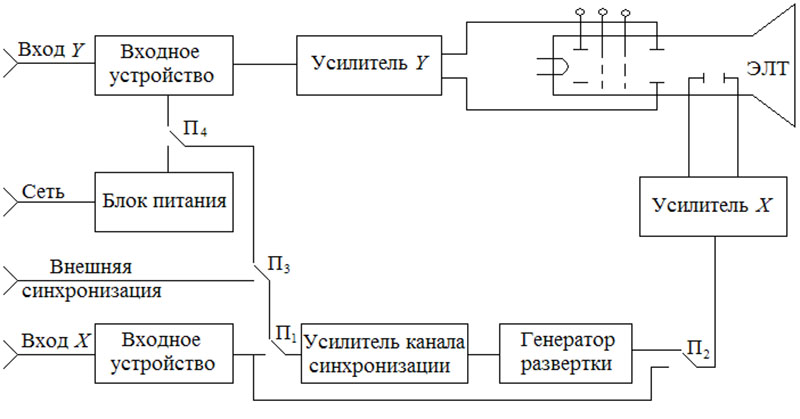
\includegraphics[width = 0.95\textwidth]{Schem_oscillograph}
			\caption{Cхема устройства осциллографа.}
			\label{fig:schem}
		\end{center}
	\end{figure}		
		
	
	
	\subsection{Принцип работы.}
	Основной элесент осциллографа -- электронно-лучевая трубка. Электронный пучок формируется системой электродов, называемой электронной пушкой: катод с нагревателем, модулятор, фокусирующий и ускоряющий аноды. Форма, размеры и расположение электродов подобраны таким образом, чтобы разгонять электроны и фокусировать пучок на экране. 
	
	На пути к экрану, сформированный пучок проходит две пары отклоняющих пластин. Две вертикальные пластины образуют плоский конденсатор, поле которого способно отклонять пучок в горизонтальном направлении. Аналогично, поле горизонтального конденсатора способно отклонять пучок в вертикальном направлении. Подавая на пластины электрическое напряжение и отслеживая траеторию пучка на экране можно анализировать входящий сигнал.
	
	\textbf{Развертка.}
	
	Так как подаваемые на пластины сигналы лежат в довольно широком диапазоне, а чувствительность трубки довольно сильно ограничена, то в конструкции осциллографа присутствуют делители и усилетели.(Рис. ~\ref{fig:schem})
	
	Для получения на экране изображения необходимо выполнение двух условий:
	
	\begin{enumerate}
		\item Подаваемое на вертикально отклоняющие пластины напряжение должно линейно завсить от сигнала.
		\item Подаваемое на горизонтально отклоняющие пластины напряжение должно линейно зависить от времени.
	\end{enumerate}
	
	В таком случае, напряжение пилообразной формы, вырабатываемое генератором, (Которое называется напряжением развертки) имеет вид, представленный на рисунке \ref{fig:voltage}.
	
	
	\begin{figure}[h]
		\begin{center}
			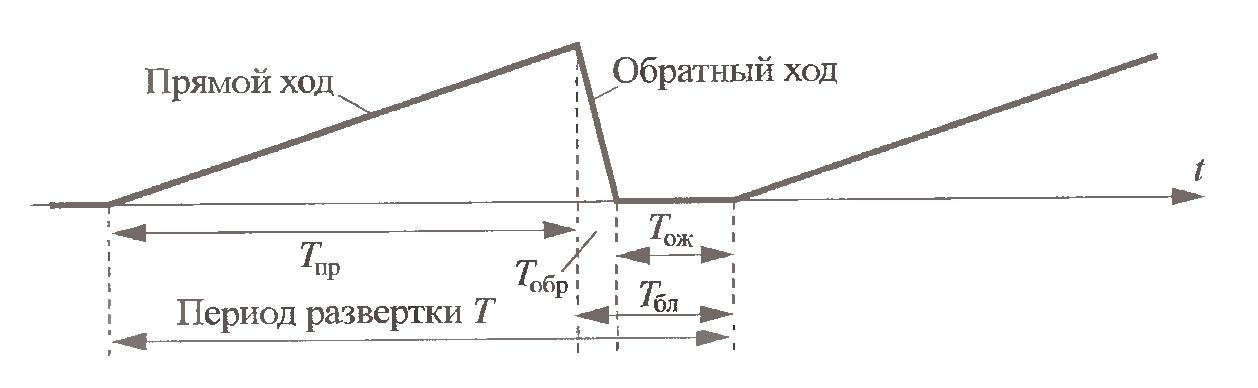
\includegraphics[width = 0.95\textwidth]{voltage_razv}
			\caption{Напряжение развертки.}
			\label{fig:voltage}
		\end{center}
	\end{figure}

	Кроме того, еще один важный процесс - синхронизация. Для получения устойчивой картины сигнала на экране необходимо, чтобы период развертки был кратен периоду самого сигнала (Рис.\ref{fig:sinchronization})
	
	\begin{figure}[h]
		\begin{center}
			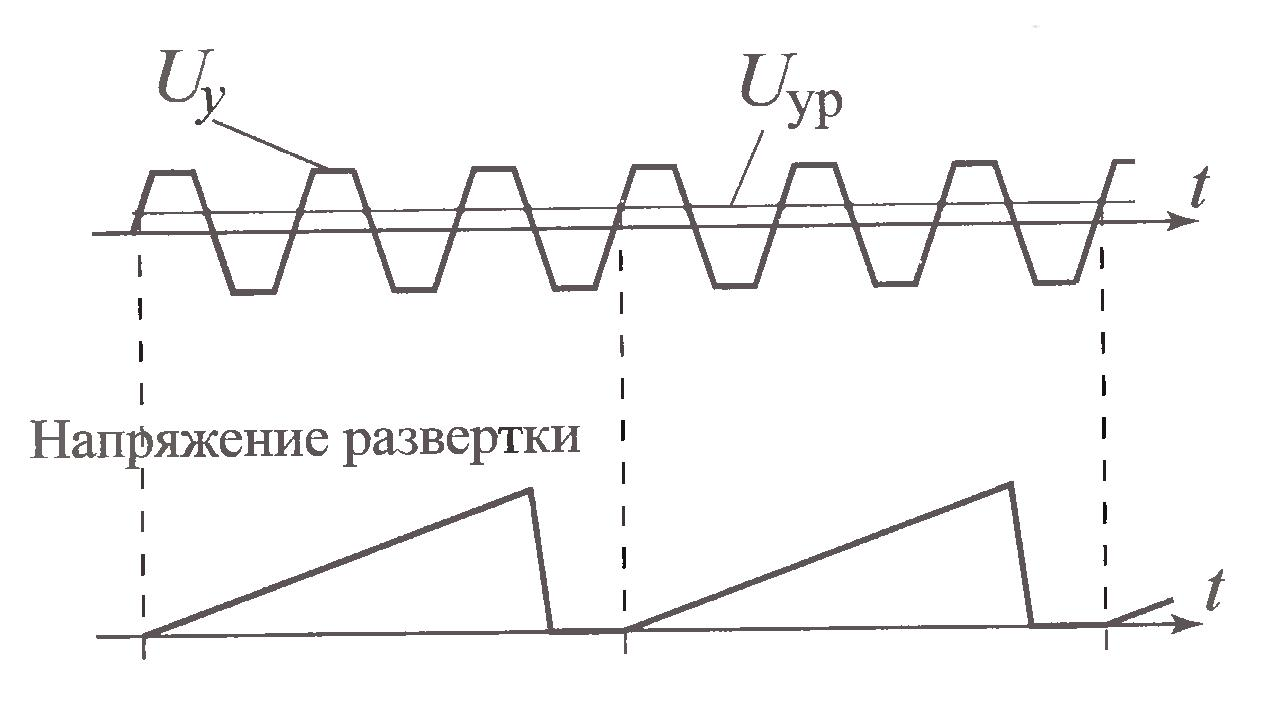
\includegraphics[width = 0.75\textwidth]{sinchronization}
			\caption{Условие наблюдения устойчивой картины сигнала на экране осциллографа.}
			\label{fig:sinchronization}
		\end{center}
	\end{figure}
\newpage
\section{Выполнение работы.}
	\subsection{Наблюдение периодического сигнала от генератора и измерение его частоты.}
	

	Необходимо получиить на экране осциллографа устойчивую картину периодического (синусоидального) сигнала. После получения картины на экране осциллографа определить период и частоту сигнала, сравнить полученные результаты с показаниями частоты на звуковом генераторе.
	
	Для получения стационарной картины используем ручки VOLTS/DIV и TIME/DIV, а также ручки POSITION и LEVEL. Получив устойчивую картину, проводим необходимые измерения. Результаты заносим в Таблицу~\ref{tab:frequency}.
		
	\begin{table}[h]
		\begin{center}
			\begin{tabular}{|l|c|c|c|c|c|c|}
				\hline
				$f_{ist}$, Гц & T, дел & TIME/DIV, mks & T, мс & f, Гц & $\delta f$, Гц & $f_{ist} - f$, Гц \\ \hline
				505 & 20 & 500  & 2     & 500   & 25    & 5  \\ \hline
				1008 & 25  & 200  & 1     & 1000  & 40    & 8 \\ \hline
				2004 & 25  & 100  & 0,5   & 2000  & 80    & 4 \\ \hline
				3002 & 35  & 50   & 0,35  & 2857  & 82    & 145 \\ \hline
				3099 & 33  & 50   & 0,33  & 3030  & 92    & 69 \\ \hline
				4006 & 25  & 50   & 0,25  & 4000  & 160    & 6 \\ \hline
				5003 & 20  & 50   & 0,2   & 5000  & 250    & 3 \\ \hline	
			\end{tabular}
			\caption{Результаты измерения частоты входного сигнала.}
			\label{tab:frequency}
		\end{center}
	\end{table}
	
	Значение величин $f,\quad \delta f $ рассчитывается по следующим формулам:
	
	\begin{center}
		\begin{spacing}{1,6}	
			$ f = \frac{1}{T} $	
	
			$ \delta f = f  \epsilon_{T},$ где $ \epsilon_{N_{T}} = \frac{\delta_{N_{T}}}{N_{T_{div}}} = \epsilon_{T}, \delta_{N_{T}} = 1 $
		\end{spacing}
	\end{center}
	
	Анализируя полученый результат, отметим следующее:
	
	\begin{enumerate}
		\item Измерение, проведенное для значения $ f_{ist} = 3002$ Гц является ошибочным. В дальнейшем, данное измерение учитывать не будем из-за очень большого отклонения. 
		\item Несмотря на довольно малые значения $ \delta f $, следует отметить, что значение $ \epsilon_{f} $ достаточно велико. Значения для различных частот занесены в таблицу \ref{tab:epsilon_frequency}.
		\item Хорошая точность обеспечивается при условии кратности измеряемой частоты величине, равной произведению $ TIME/DIV * N_{div_{T}} $
		\item Данный метод позволяет добиться точности измерения частоты входящего сигнала 5$\%$ от значения измеряемой величины.
	\end{enumerate}
	
	\begin{table}[h]
		\begin{center}
			\begin{tabular}{|l|l|l|l|l|l|l|l|}
				\hline
				$\epsilon_{f}$ & 0,05 & 0,04 & 0,04 & 0,03 & 0,03 & 0,04 & 0,05 \\ \hline
				    $f,$ Гц    & 500  & 100  & 2000 & 2857 & 3030 & 4000 & 5000 \\ \hline
			\end{tabular}
			\caption{Значения относительной погрешности определения частоты для различных частот.}
			\label{tab:epsilon_frequency}
		\end{center}
	\end{table}
	
	
	\subsection{Измерение амплитуды сигнала.}
	
	С помощью вертикальной шкалы осциллографа проведем измерение амплитуды сигнала. Для этого установим значение частоты входного сигнала осциллографа 1 кГц, затем измерим отношение $ \frac{U_{max}}{U_{min}} , $ которые способен выдавать генератор. Изменение напряжение входного сигнал аобеспечим с помощью кнопки ATT - 20dB, которая уменьшает амплитуду в 10 раз.
	
	Формула, которая описывает происходящие изменения:
	$$ \beta_{21} = 20 \lg\frac{U_{2}}{U_{1}} $$
	
	Проверим ее истинность: Измерим значения $ U_{max},U_{min},$ а также определим $ \beta_{21}.$ Полученный результат занесем в таблицу \ref{tab:amplitude}.
	
		
	\begin{table}[h]
		\begin{center}
			\begin{tabular}{|c|c|c|c|c|c|c|c|c|c|}
				\hline
				$U_{max},$ В & $U_{min},$ В & $\delta U_{max}$ & $\delta U_{min}$ & $\epsilon_{U_{max}}$ & $\epsilon_{U_{min}}$ & $\beta_{teor}$ & $\beta$ & $\epsilon_{beta}$ & $\delta \beta$ \\ \hline
				26    & 2,8   & 1  & 0,1 & 0,04 & 0,04 & 20 & 19,4 & 0,02 & 0,5\\ \hline
			\end{tabular}
			\caption{Результаты измерения амплитуды входного сигнала.}
			\label{tab:amplitude}
		\end{center}
	\end{table}
	
	Величина $\delta_{beta}$ вычисляется по формуле: $$ \delta_{beta} = \sqrt{\left(\frac{20}{U_{max}\ln10}\right)^2 + \left(\frac{20}{U_{min}\ln10}\right)^2} $$
	
	Сравнивая полученное значение $ \beta = 19,4 \pm 0,7 $ с теоретически рассчитанным $ \beta_{teor} = 20 , $ можно сказать, что теоретическое соотношение выполняется при заданной частоте входного сигнала.
	
	
	\subsection{Изиерение амплитудно-частотной характеристики осциллографа.}
	
	\textit{Амплитудо-частнотной характеристикой} (АЧХ) измерительного прибора называют зависимость амплитуды измеряемого
сигнала от частоты сигнала, подаваемого на вход.  Проведем измерение АЧХ для двух состояний канала осциллографа во всем диапазоне частот.

	Формула, которая позволяет определить АЧХ:
	
	$$ K(f) = \frac{U(f)}{U_{0}} $$
		
		Проведем измерения при $ U_{0,DC} = 20 $ дел, $ U_{0,AC} = 20 $ дел. Результаты занесем в таблицу  \ref{tab:amplfreqparamAC_DC}. На основе полученных данных построим график.
		
		\begin{table}[t]
			\begin{center}
				\begin{tabular}{|c|c|c|c|c|c|}
				\hline
f, Гц & $\lg{f}$  & $2U_{DC}$, дел & $K_{DC} = \frac{U_{DC}}{U_{0}}$ & $2U_{AC}$, дел & $K_{AC} = \frac{U_{AC}}{U_{0}}$ \\ \hline
5   & 0,699 & 19  & 0,95 & 17  & 0,85    \\ \hline
10  & 1,000 & 20  & 1 & 19  & 0,95    \\ \hline
20  & 1,301 & 20  & 1 & 20 & 1 \\ \hline
50  & 1,699 & 20   & 1 & 20  & 1 \\ \hline
$10^{2}     $& 2,000 & 20  & 1 & 20  & 1 \\ \hline
$2*10^{2}   $& 2,301 & 20  & 1 & 20  & 1 \\ \hline
$5*10^{2}   $& 2,699 & 20  & 1 & 20  & 1 \\ \hline
$10^{3}     $& 3,000 & 20  & 1 & 20  & 1 \\ \hline
$2*10^{3}   $& 3,301 & 20  & 1 & 20  & 1 \\ \hline
$5*10^{3}   $& 3,699 & 20  & 1 & 20  & 1 \\ \hline
$10^{4}     $& 4,000 & 20  & 1 & 20  & 1 \\ \hline
$2*10^{4}   $& 4,301 & 20  & 1 & 20  & 1 \\ \hline
$5*10^{4}   $& 4,699 & 20  & 1 & 20  & 1 \\ \hline
$10^{5}     $& 5,000 & 20  & 1 & 20  & 1 \\ \hline
$2*10^{5}   $& 5,301 & 20  & 1 & 20  & 1 \\ \hline
$5*10^{5}   $& 5,699 & 20  & 1 & 20  & 1 \\ \hline
$10^{6}     $& 6,000 & 20  & 1 & 19  & 0,95    \\ \hline
$1,5*10^{6} $& 6,176 & 20  & 1 & 19  & 0,95    \\ \hline
$2*10^{6}   $& 6,301 & 20  & 1 & 19  & 0,95    \\ \hline
$2,5*10^{6} $& 6,398 & 19  & 0,95    & 19  & 0,95    \\ \hline
$3*10^{6}   $& 6,477 & 19  & 0,95    & 19  & 0,95    \\ \hline
$3,5*10^{6} $& 6,544 & 18  & 0,9     & 18  & 0,9     \\ \hline
$4*10^{6}   $& 6,602 & 18  & 0,9     & 18  & 0,9     \\ \hline
$4,5*10^{6}$ & 6,653 & 18  & 0,9     & 18  & 0,9     \\ \hline
$5*10^{6}$   & 6,699 & 18  & 0,9     & 18  & 0,9     \\ \hline
\end{tabular}
\caption{Значение K дя различных частот для закрытого и открытого канала.}
\label{tab:amplfreqparamAC_DC}
\end{center}
\end{table}


\begin{figure}[h!]
	\begin{center}
		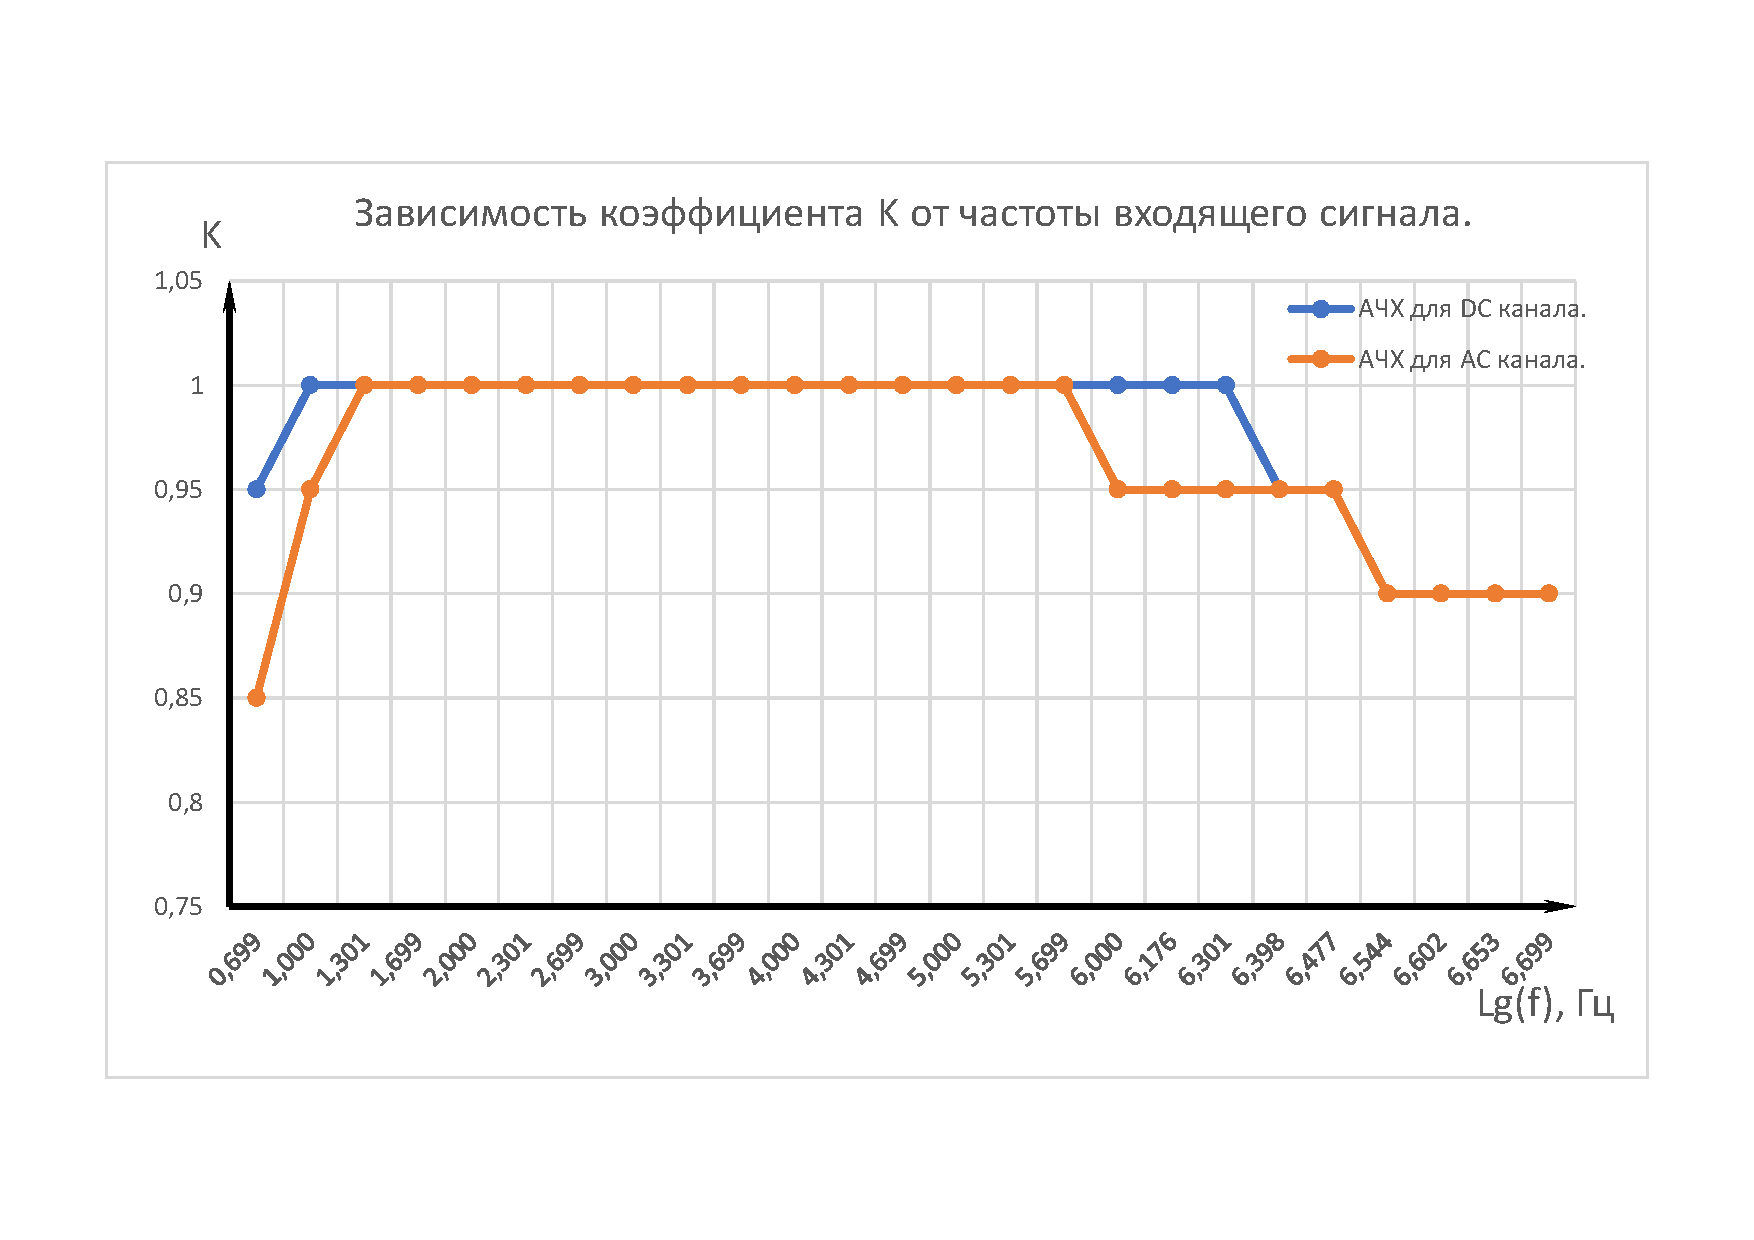
\includegraphics[width = 0.76\textwidth]{Amplitude-frequency-characteristic_AC_DC_graph}
		\label{fig:Amplitude-frequency-characteristic_AC_DC_graph}
	\end{center}
\end{figure}
		
	\subsection{Изучение влияния АЧХ на искажение сигнала.}
	
	Проверим, каким образом АЧХ влияет на искажение прямоугольного сигнала, подаваемого на закрытый вход AC - меандра. Для этого получим устойчивую картину прямоугольного сигнала для частоты $ f = 1$ кГц. Затем, изменяя частоту входного сигнала получим картины меандров для различных частот.
	
	Из-за искажения, вызванного АЧХ осциллографа, при достаточно больших частотах, вероятнее всего будет наблюдаться картина, изображенная на рисунке \ref{fig:meandr_teor}. Сигнал приобретает выбросы и всплески в первую очередь, из-за индуктивности монтажа. Кроме того, передний и задний фронты сигнала возникают не сразу, а имеют какое-то время нарастания и спада, из-за чего они наклонены относительно вертикальной линии.Этот наклон обусловлен частотными свойствами микросхем и транзисторов: чем более высокочастотный транзистор, тем менее завалены фронты импульсов.
	\begin{figure}[h!]
		\begin{center}
			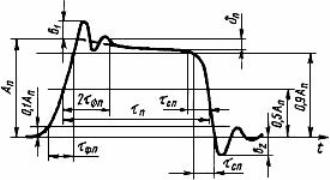
\includegraphics[height = 0.14\textheight]{meandr_illustration}
			\caption{Теоретическая картина сигнала меандра, искаженного осциллографом.}
			\label{fig:meandr_teor}
		\end{center}			
	\end{figure}
	
	
	На рисунках \ref{ris:meandr_100Hz} - \ref{ris:meandr_4MHz} представленны картины сигналов для различных значений частоты.
	\begin{figure}[h!]
		\begin{center}
			\begin{minipage}[h]{0.32\linewidth}
				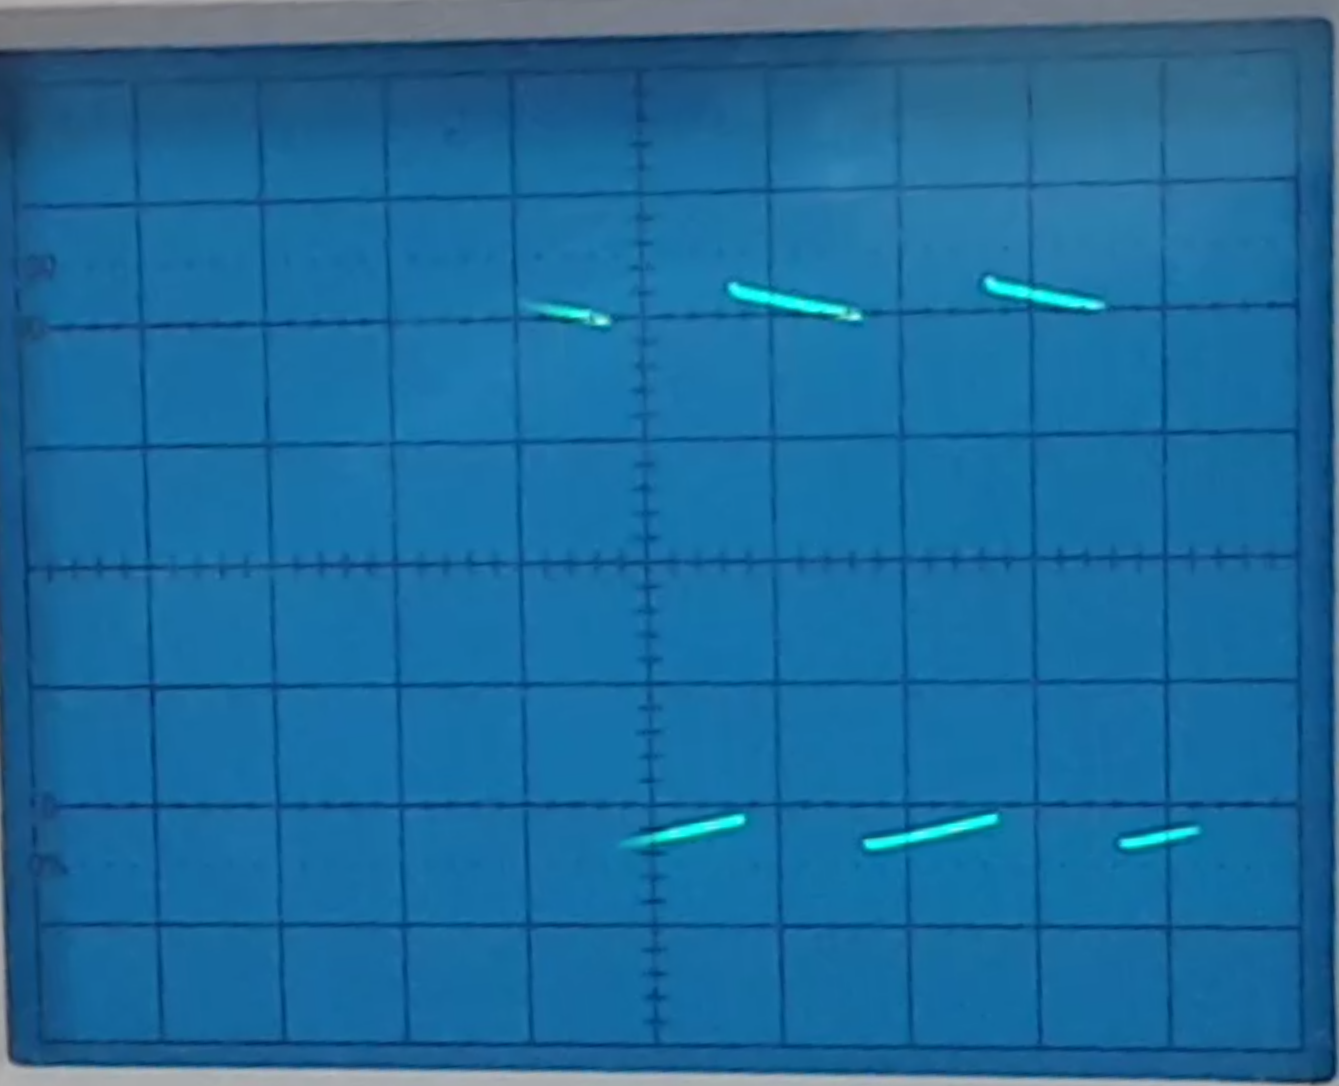
\includegraphics[width=1\linewidth]{meandr_100Hz}
				\caption{100 Гц.} %% подпись к рисунку
				\label{ris:meandr_100Hz} %% метка рисунка для ссылки на него
			\end{minipage}
		\hfill
			\begin{minipage}[h]{0.32\linewidth}
				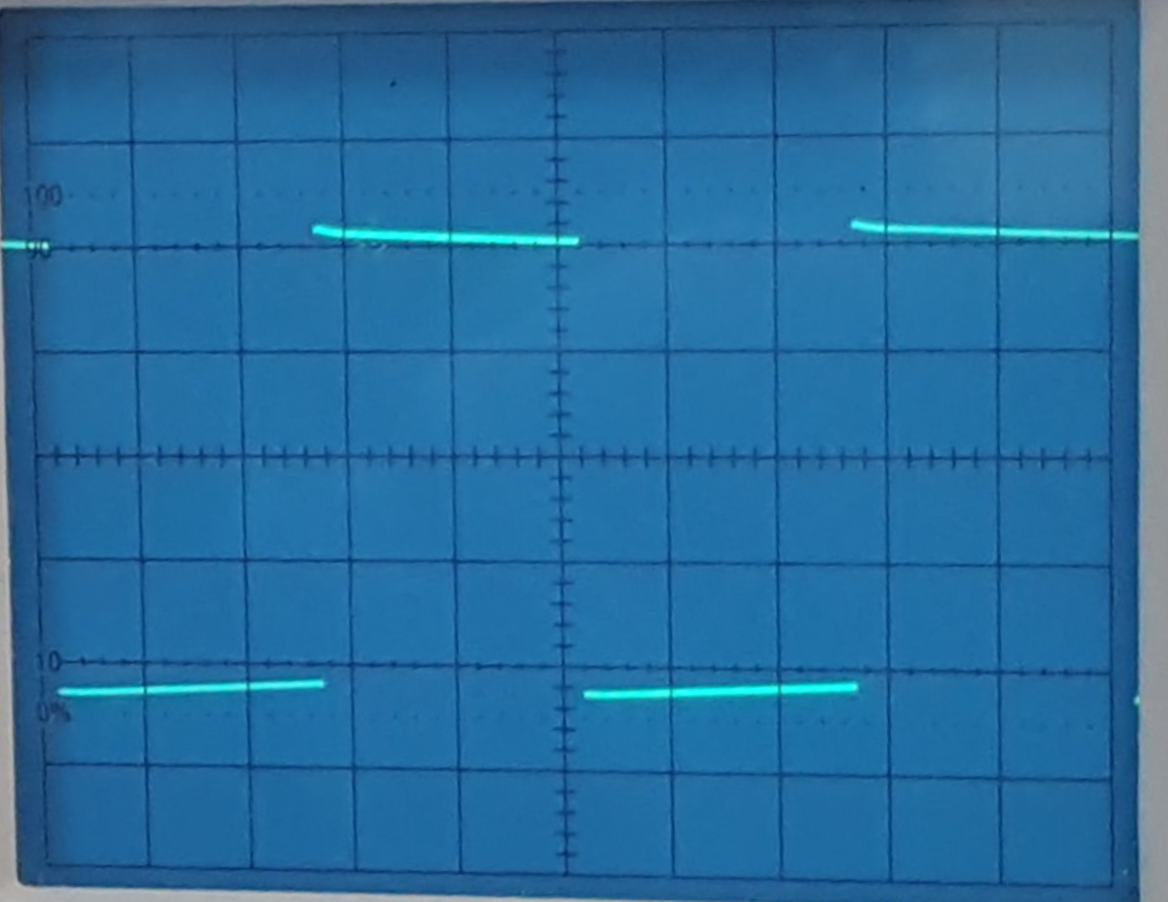
\includegraphics[width=1\linewidth]{meandr_200Hz}
				\caption{200 Гц.}
				\label{ris:meandr_200Hz}
			\end{minipage}
		\hfill
			\begin{minipage}[h]{0.32\linewidth}
				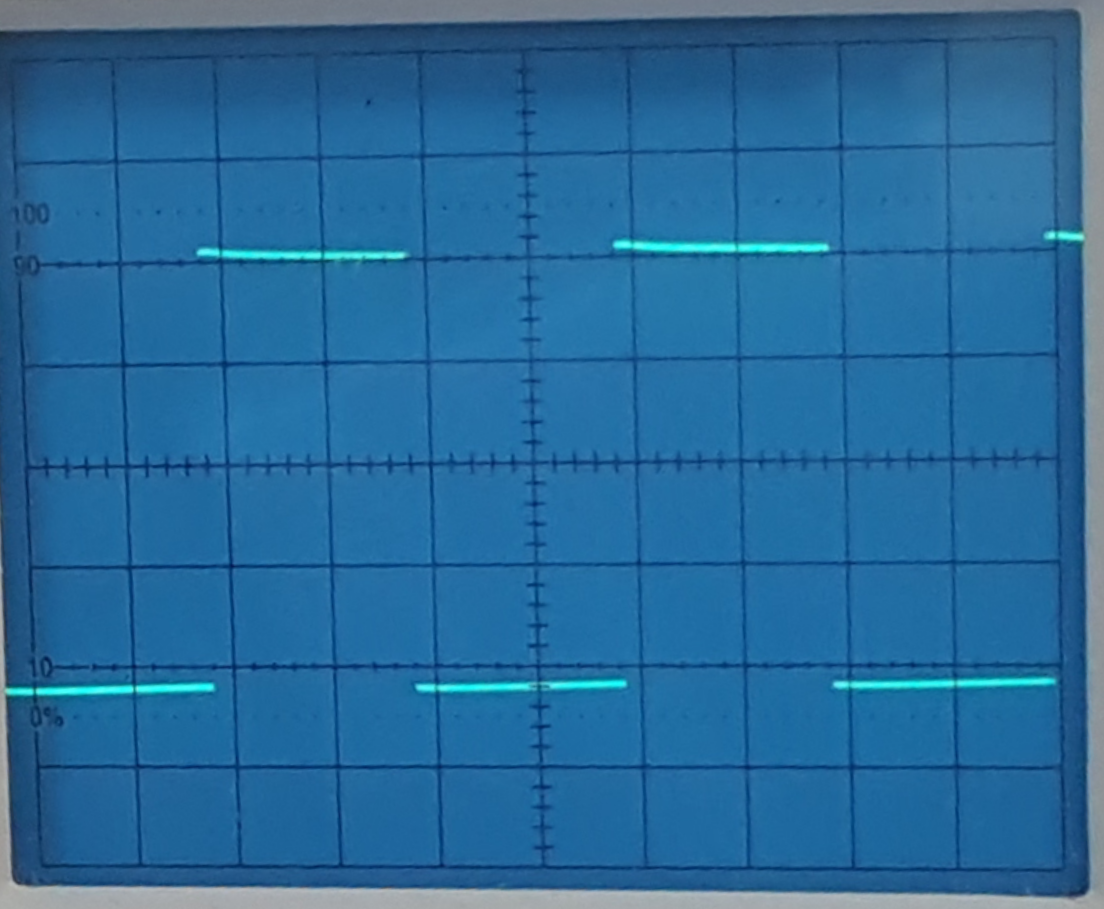
\includegraphics[width=1\linewidth]{meandr_500Hz}
				\caption{500 Гц.} %% подпись к рисунку
				\label{ris:meandr_500Hz} %% метка рисунка для ссылки на него
			\end{minipage}
		\end{center}
		\begin{center}
			\begin{minipage}[h]{0.32\linewidth}
				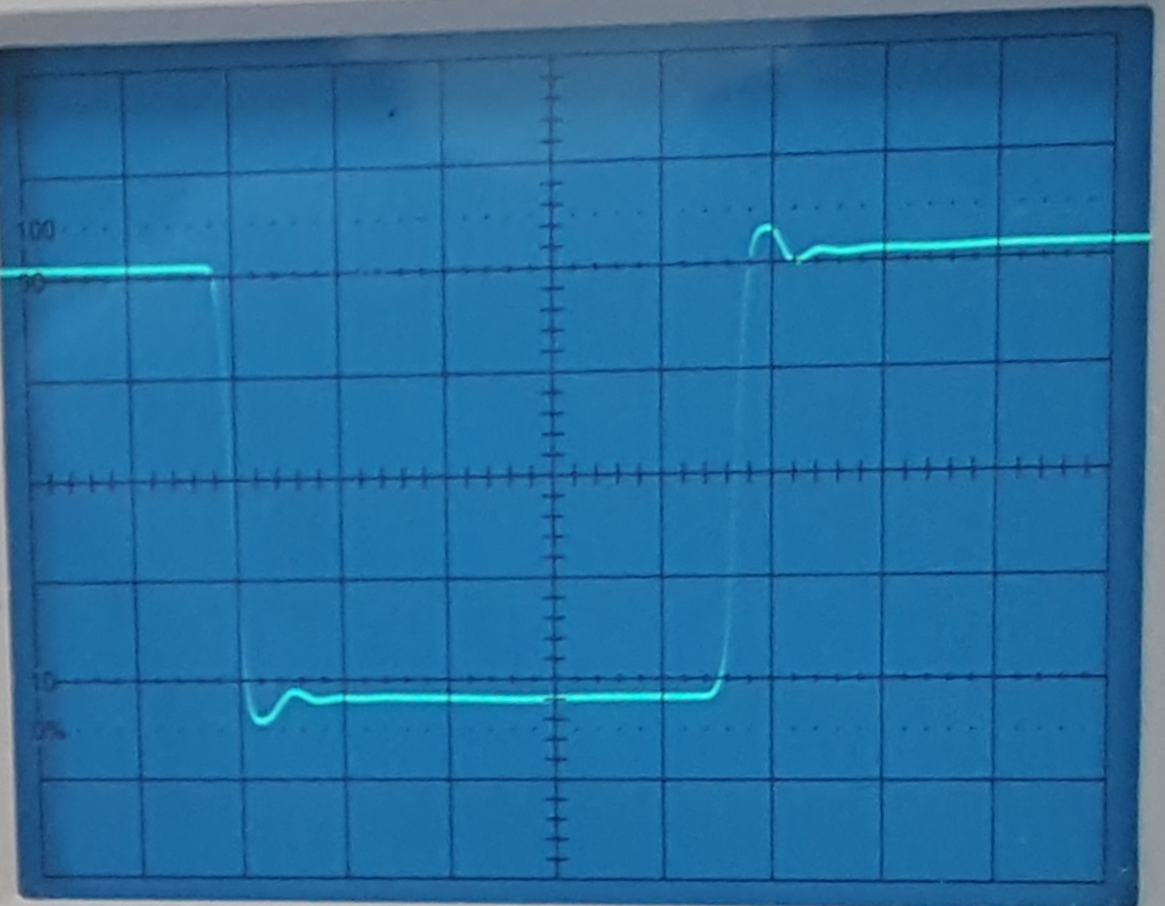
\includegraphics[width=1\linewidth]{meandr_500kHz}
				\caption{500 кГц.}
				\label{ris:meandr_500kHz}
			\end{minipage}
		\hfill
			\begin{minipage}[h]{0.32\linewidth}
				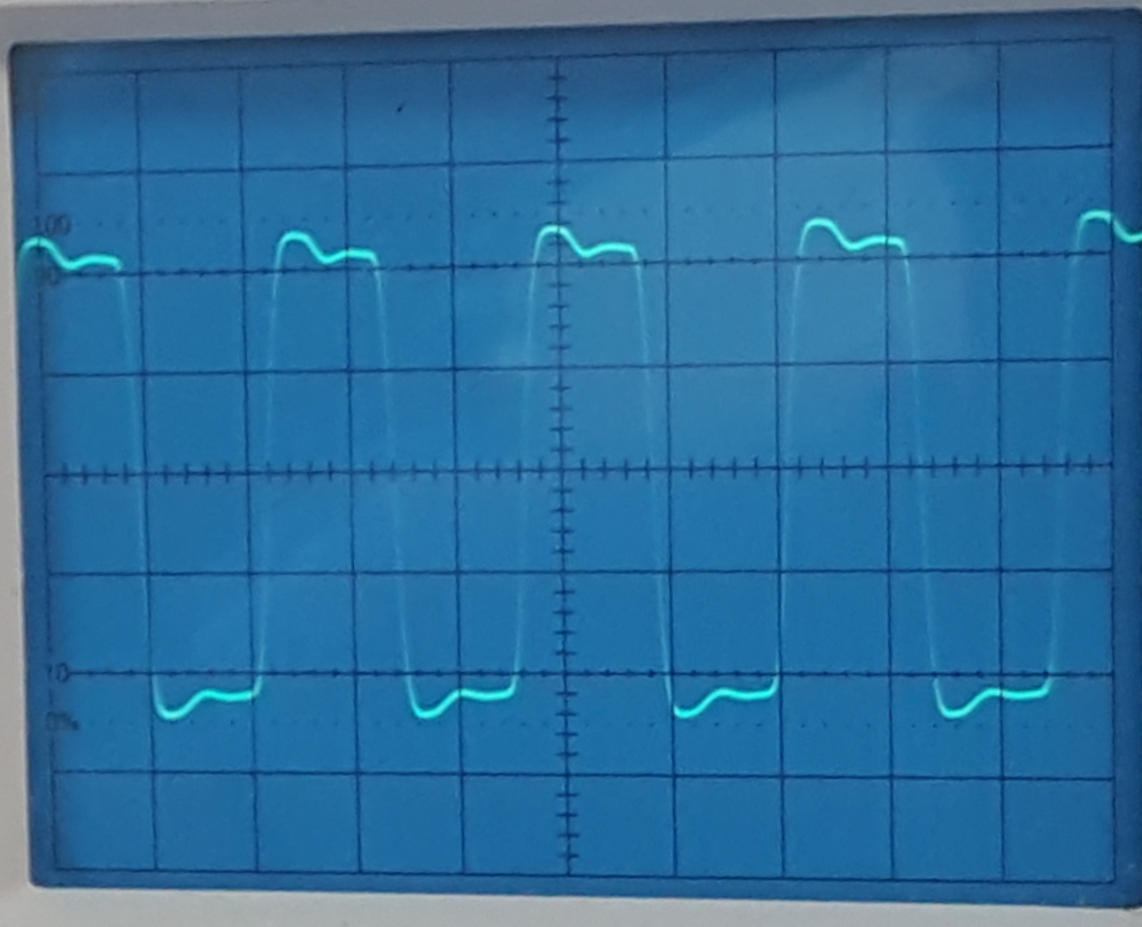
\includegraphics[width=1\linewidth]{meandr_2MHz}
				\caption{2 МГц.} %% подпись к рисунку
				\label{ris:meandr_2MHz} %% метка рисунка для ссылки на него
			\end{minipage}
		\hfill
			\begin{minipage}[h]{0.32\linewidth}
				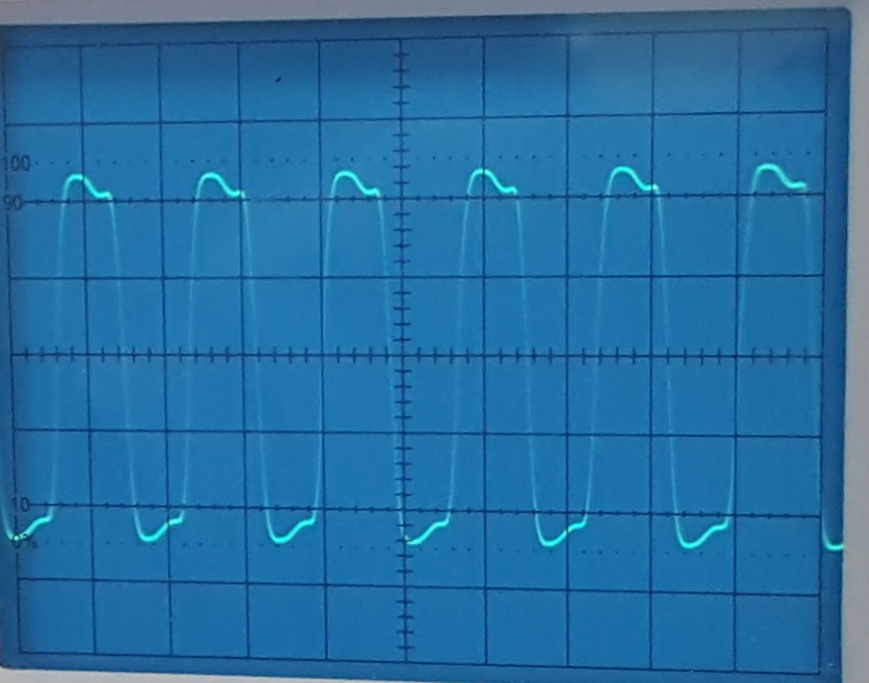
\includegraphics[width=1\linewidth]{meandr_3MHz}
				\caption{3 МГц.}
				\label{ris:meandr_3MHz}
			\end{minipage}
		\end{center}
		\begin{center}
			\begin{minipage}[lh]{0.32\linewidth}
				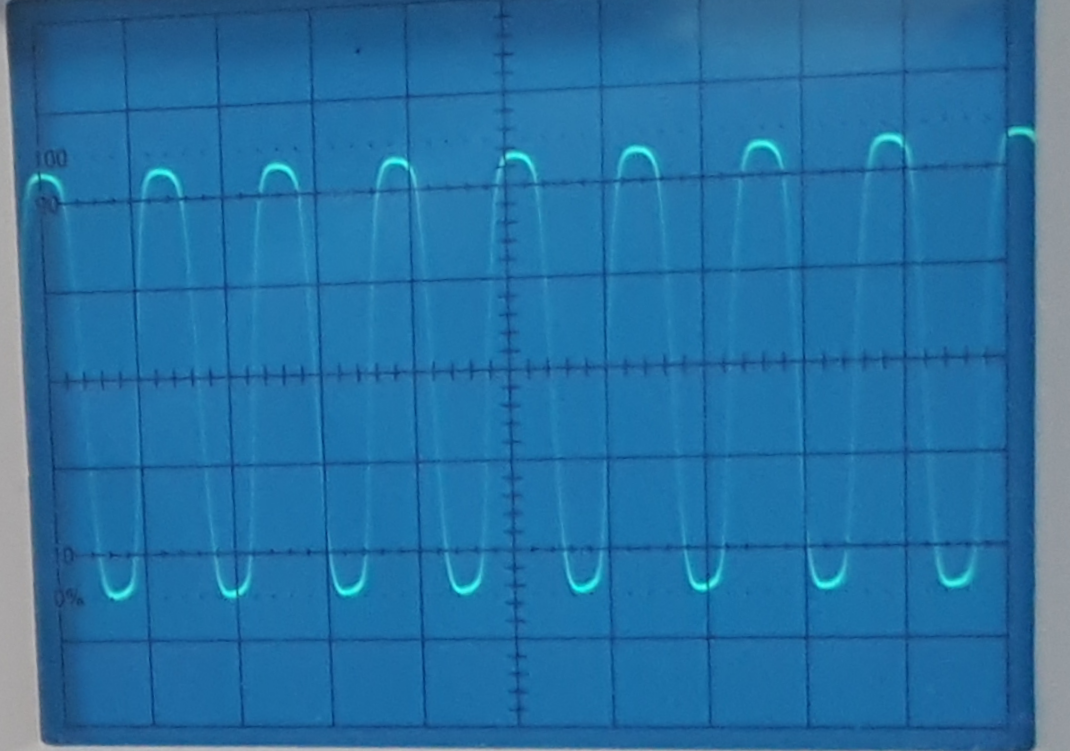
\includegraphics[width=1\linewidth]{meandr_4MHz}
				\caption{4 МГц.} %% подпись к рисунку
				\label{ris:meandr_4MHz} %% метка рисунка для ссылки на него
			\end{minipage}
		\hfill	
		\end{center}
	\end{figure}
	
	По полученым картинам можно сказать, что наибольшее искажение происходит в диапазонах низких ($\leq 100$ Гц) и высоких ($\geq 1$ МГц) частот. Кроме того, полученые картины в достаточно большой степени похожи на картину, предсказанную теоретически (Рис. \ref{fig:meandr_teor})
	
	Опишем характер изменений:
	
	Для низких частот (Рис. \ref{ris:meandr_100Hz}) сигнал превращается в некоторое семейство кривых, стремящихся к оси времени, и имеющих пик слева. Кривые довольно плавные, однако при повышении частоты стремление кривой к оси уменьшается, начинает формироваться ступень. Для частот порядка 500 Гц кривые практически полностью становятся отрезками прямых, имеющих незначительный наклон к оси времени. (Рис. \ref{ris:meandr_500Hz}). 
	
	Для средних частот картина довольно хорошо описывется теоретическими представлениями об искажении сигнала (Рис. \ref{fig:meandr_teor}).
	
	Для высоких частот наблюдается сглаживание ломанной, ступенчатой кривой. Как видно на Рис. \ref{ris:meandr_4MHz} для больших частот сигнал уже мало похож на ступенчатую ломанную.
	\subsection{Измерение разности фазово-частотных характеристик каналов осциллографа.}
		
	Проведем измерение разнасти фаз входящих сигналов. Для подготовки к измерениям выполним следующие действия:
	\begin{enumerate}
		\item Подадим синусоидальный сигнал частотой $f = 1$ кГц с помощью тройника на каналы X и Y. Внутреннюю развертку включим в режим X-Y.В этом режиме отклонение луча на экране пропорционально  подаваемым на каналы напряжениям $$Y(t) = k_{y}U_{y}(t);  \quad X(t) = k_{x}U_{x}(t);$$ где коэффициенты
масштаба $k_{x}$, $k_{y}$ определяются положениями ручек VOLTS/DIV.
		\item Используя ручки VOLTS/DIV получим на экране вырожденный эллипс, направленный под углом $45^{o}$ к оси X.
		\item Изменяя частоту генератора $ f $ во всем доступном диапазоне найдем участки, на которых изображение на экране переходит из отрезка в невырожденный эллипс. На этих участках проведем подробное измерение разности фаз $\Delta\phi(f)$ между каналами X и Y в зависимости от частоты.
		
		Траектория луча на экране представляет собой эллипс (Рис.~\ref{fig:ellipse}), который можно описать уравнениями:
		
	\begin{figure}[h]
		\begin{center}
			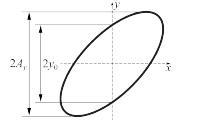
\includegraphics[width = 0.4\textwidth]{Ellipse_for_delta_phases}
			\caption{Устойчивая картина невырожденного эллипса на экране осциллографа.}
			\label{fig:ellipse}		
		\end{center}
	\end{figure}
		
	$$ x(t) = A_{x}\sin(\omega t + \phi_{x}); \qquad y(t) = A_{y}\sin(\omega t + \phi_{y}) $$
	
	Разность фаз $ \Delta\phi = \phi_{x} - \phi_{y} $ можно вычислить с помощью формулы:
	
	$$ \sin|\Delta\phi| = \left|\frac{y_{0}}{A}\right| $$
	
	Тогда для определения $\Delta\phi$  получаем формулы:
		
	$$\Delta\phi = \arcsin\left|\frac{y_{0}}{A}\right|$$		
				
	$$\Delta\phi = \pi - \arcsin\left|\frac{y_{0}}{A}\right|$$
		
		
	
	
		\item Результаты измерений занесем в таблицы ~\ref{tab:delta_phases_DC}, \ref{tab:delta_phases_AC}. По результатам измерений построим график. (Рис. \ref{fig:grafic_delta_phases}).
	\end{enumerate}
	
	\begin{table}[]
	\begin{center}
		\begin{tabular}{|c|c|c|c|c|c|}
			\hline
			$ f * 10^{6}$ Гц      & lg f & |2y0|, дел & |2A|, дел & $\arcsin\left|\frac{y0}{A}\right|$, рад & $\Delta\phi$, рад \\ \hline
			0,8  & 5,91 & 8     & 20   & 0,41   & 0,41     \\ \hline
			1,0 & 6,00 & 10    & 20   & 0,52   & 0,52     \\ \hline
			1,2 & 6,08 & 12    & 20   & 0,64   & 0,64     \\ \hline
			1,5 & 6,18 & 14    & 20   & 0,78   & 0,78     \\ \hline
			1,7 & 6,23 & 16    & 19   & 1,00   & 1,00     \\ \hline
			1,9 & 6,28 & 17    & 19   & 1,11   & 1,11     \\ \hline
			2,5 & 6,40 & 19    & 19   & 1,57   & 1,57     \\ \hline
			3,0 & 6,48 & 17    & 19   & 1,11   & 2,03     \\ \hline	
			3,2 & 6,51 & 16    & 19   & 1,00   & 2,14     \\ \hline	
			3,4 & 6,53 & 14    & 19   & 0,83   & 2,31     \\ \hline
			3,7 & 6,57 & 12    & 19   & 0,68   & 2,46     \\ \hline
			3,9 & 6,59 & 10    & 19   & 0,55   & 2,59     \\ \hline
			4,1 & 6,61 & 8     & 19   & 0,43   & 2,71     \\ \hline
			4,3 & 6,63 & 7     & 19   & 0,38   & 2,76     \\ \hline
			4,5 & 6,65 & 6     & 19   & 0,32   & 2,82     \\ \hline
			4,8 & 6,68 & 5     & 19   & 0,27   & 2,88     \\ \hline
			5,0 & 6,70 & 3     & 19   & 0,16   & 2,98     \\ \hline
		\end{tabular}
		\caption{Результаты измерения разности фаз сигналов для открытого канала.}
		\label{tab:delta_phases_DC}
	\end{center}
	\end{table}
	
	\begin{table}[]
	\begin{center}
		\begin{tabular}{|c|c|c|c|c|c|}
			\hline
			$ f * 10^{6}$ Гц      & lg f & |2y0|, дел & |2A|, дел & $\arcsin\left|\frac{y0}{A}\right|$, рад & $\Delta\phi$, рад \\ \hline
			0,8  & 5,91 & 8     & 20   & 0,41   & 0,41     \\ \hline
			1,0 & 6,00 & 10    & 20   & 0,52   & 0,52     \\ \hline
			1,2 & 6,08 & 12    & 20   & 0,64   & 0,64     \\ \hline
			1,5 & 6,18 & 14    & 20   & 0,78   & 0,78     \\ \hline
			1,7 & 6,23 & 16    & 19   & 1,00   & 1,00     \\ \hline
			1,9 & 6,28 & 17    & 19   & 1,11   & 1,11     \\ \hline
			2,5 & 6,40 & 19    & 19   & 1,57   & 1,57     \\ \hline
			3,0 & 6,48 & 17    & 19   & 1,11   & 2,03     \\ \hline	
			3,2 & 6,51 & 16    & 19   & 1,00   & 2,14     \\ \hline	
			3,4 & 6,53 & 14    & 19   & 0,83   & 2,31     \\ \hline
			3,7 & 6,57 & 12    & 19   & 0,68   & 2,46     \\ \hline
			3,9 & 6,59 & 10    & 19   & 0,55   & 2,59     \\ \hline
			4,1 & 6,61 & 8     & 19   & 0,43   & 2,71     \\ \hline
			4,3 & 6,63 & 7     & 19   & 0,38   & 2,76     \\ \hline
			4,5 & 6,65 & 6     & 19   & 0,32   & 2,82     \\ \hline
			4,8 & 6,68 & 5     & 19   & 0,27   & 2,88     \\ \hline
			5,0 & 6,70 & 3     & 19   & 0,16   & 2,98     \\ \hline
		\end{tabular}
		\caption{Результаты измерения разности фаз сигналов для закрытого канала.}
		\label{tab:delta_phases_AC}
	\end{center}
	\end{table}
	
	
	
	\begin{figure}
		\begin{center}
			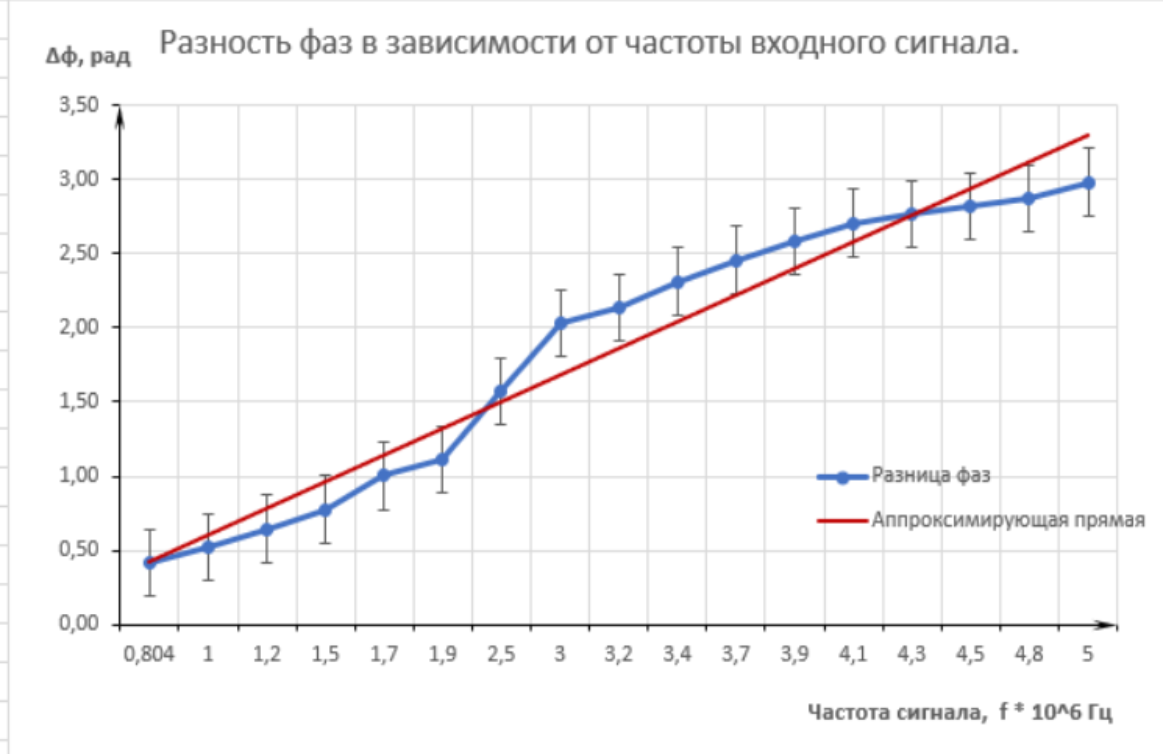
\includegraphics[width = 0.75\textwidth]{Grafic_delta_phases}
			\caption{График зависимости разности фаз входящих сигналов в зависимоти от частоты.}
			\label{fig:grafic_delta_phases}
		\end{center}
	\end{figure}
	
	
	\newpage
	
	\subsection{Наблюдение фигур Лиссажу.}

	Для наблюдения фигур Лиссвжу необходимо подать на 2 входа осциллографа 2 сигнала различной частоты (Для наблюдения фигур необходимо, чтобы частоты сигналов были соотносились как целые числа).
	
	После получения устойчивой картины фигуры Лиссажу, с помощью изображения можно определить соотношение частот входных сиогналов. Для определения соотношения необходимо провести 2 произвольные линии, параллельные осям и не пересекающие фигуру в узловых точках, затем посчитать количество точек пересечения данных прямых с фигурой. отношение чисел точек пересечния -- есть искомое соотношение между частотами.
	
	на рисунке ~\ref{fig:Lissajг_figure} представлены некоторые фигуры, которые можно получить при заданных соотношениях частот и разницы фаз входящих сигналов.
	
	\begin{figure}
		\begin{center}
			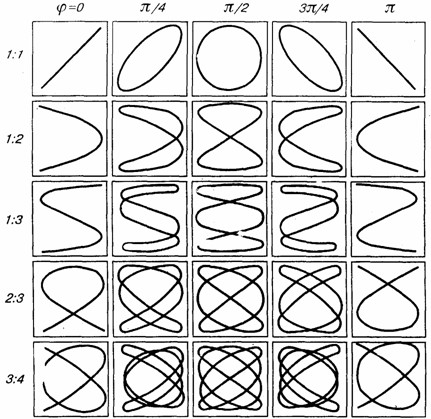
\includegraphics[width = 0.9\textwidth]{Lissaju_figure_modificed}
			\caption{Вид фигур Лиссажу для некоторых соотношений частот и заданной разности фаз входных сигналов}
			\label{fig:Lissajг_figure}
		\end{center}
	\end{figure}
	
\newpage


\section{Результаты.}

	\begin{enumerate}
	\item Во время проведения данной работы был изучен электронный осциллограф -- строение и принцип его действия.
	\item При помощи осциллографа был исследован периодичесикий сигнал, был определен период исследуемого сигнала с приемлемой точностью, (Максимальная относительная погрешность измерения равна 5$\%$).
	\item При помощи осциллографа была измерена амплитуда входящего сигнала, была проверена теоретическая формула интернсивности сигнала. Сравнивая полученное значение $ \beta = 19,4 \pm 0,7 $ с теоретически рассчитанным $ \beta_{teor} = 20 , $ можно сказать, что теоретическое соотношение выполняется при заданной частоте входного сигнала.
	\item Для данной модели осциллографа была определена зависимость АЧХ от частоты входного сигнала. Было проанализировано влияние данной зависимости на искажение сигнала.
	\item Было проведено измерение разности фазово-частотных характеристик каналов осциллографа. Анализ результатов показал, что разность ФЧХ между каналами осциллографа отсутствует на частотах $< 10^{5}$ Гц. (ФЧХ идентична для двух каналов осциллографа.)
	\item При помощи осциллографа были получены изображения фигур Лиссажу. На практике были подтверждены методы определения соотношения между частотами сигналов, образующих фигуры Лиссажу.
	\end{enumerate}



\end{document}
